\documentclass{thesisclass}
\usepackage[english]{babel}
\usepackage{graphicx} 											
\DeclareGraphicsExtensions{.pdf,.png,.jpg}								
\usepackage[natbibapa]{apacite}
\usepackage{booktabs}
\usepackage{tabularx}
\usepackage{amsmath}
\usepackage{amssymb}
\usepackage{amstext}
\usepackage{amsthm}
\usepackage[]{todonotes}
\usepackage{etoolbox}
\makeatletter
\makeatother
\usepackage{chngcntr}
\makeatletter
\makeatother
\usepackage{mathptmx}
\setkomafont{disposition}{\bfseries}


\newcommand{\type}{Project Documentation} 
\newcommand{\group}{Finn Kock, Alejandro Castilla, Sergio Pajuelo, Robert Eggert}
\newcommand{\mytitle}{SeQG - A Security Question Generator as a Webapplication}
\newcommand{\course}{Practical Course Usable Security}

\newcommand{\reviewerone}{Dr. Vikrotija Paneva and Doruntina Murtezaj}
\newcommand{\prof}{Prof. Florian Alt}
\newcommand{\timeend}{30.07.2025}
\newcommand{\submissiontime}{30.07.2025}

\hypersetup{
 pdfauthor={\group},
 pdftitle={\mytitle},
 pdfsubject={\type},
 pdfkeywords={\type}
}

\begin{document}

\begin{titlepage}
	\begin{textblock}{10}[0,0](10,2.5)
	\end{textblock}
	\changefont{ppl}{m}{n}
	\vspace*{3cm}
	\begin{center}
		\Huge{\mytitle}
		\vspace*{1.6cm}\\ % reduce vspace if title page spreads over two pages
		\Large{
			\type\\of
		}\\
		\vspace*{1cm}
		\huge{\group}\\
		\vspace*{1cm} % reduce vspace if title page spreads over two pages
		\Large{
			{Ludwig-Maximilians-Universität München}
			\\
			\course
		}
	\end{center}
	\vspace*{1.8cm} % reduce vspace if title page spreads over two pages
	\Large{
		\begin{center}
			\begin{tabular}[ht]{l c l}

				Reviewer: & \hfill  & \reviewerone\\
                Professor: & \hfill & \prof
			
			\end{tabular}
		\end{center}
	}
	
	
	\vspace{1.8cm} % reduce vspace if title page spreads over two pages
	\begin{center}
		\timeend
	\end{center}
	
	
	
\end{titlepage}
\clearpage
% Inside the main nothing but the Title is allowed! this way we keep it clean :)
\chapter{Index}
...
\chapter{Introduction}
This is the intro to our project
\chapter{Frontend}

Frontend definition

\section{General Setup}


\section{URL Routing}
For URL navigation, we decided to use file based routing, which is a common practice in modern web applications.
In our specific case, we used the TanStack Router library.
This approach allows us to modularize our application into clear and structured URLs.
We can clearly define which component is in use, when a certain URL is accessed, which makes the code better maintainable and more understandable.


\section{Main Screen}
\begin{figure}[H]
    \centering
    
\includegraphics[width=0.8\textwidth]{images/MainScreen1.png}
    \caption{Main Screen}
\end{figure}

When the system is offline, the display shows a static screen where \textbf{security tips and news} are 
dynamically fetched by the LLM. These messages, shown in Figure 2.1, are designed to catch users’ attention 
and encourage them to engage with \textbf{SeQG} and learn more about \textbf{cybersecurity}.

\begin{figure}[H]
    \centering
    
\includegraphics[width=0.4\textwidth]{images/MainScreenCharacter1.png}
    
\includegraphics[width=0.4\textwidth]{images/MainScreenCharacter2.png}
    \caption{Characters for Mode selection}
\end{figure}
When a user approaches the display and taps the screen, \textbf{two mode characters} appear, each accompanied 
by a short explanation of their functionality, as to be seen in Figure 2.3.
\section{Welcome Screens}

\begin{figure}[H]
    \centering
     
\includegraphics[width=0.6\textwidth]{images/WelcomeScreen.png}
     \caption{Main When connected}
\end{figure}
When the user scans the QR code with their device, a screen will appear allowing them to leave the 
session remotely without needing to interact directly with the public display. While connected, 
a \textbf{session token} linked to the user's device is stored on the server, preventing other 
users from interfering with the session.

\begin{figure}[H]
    \centering
    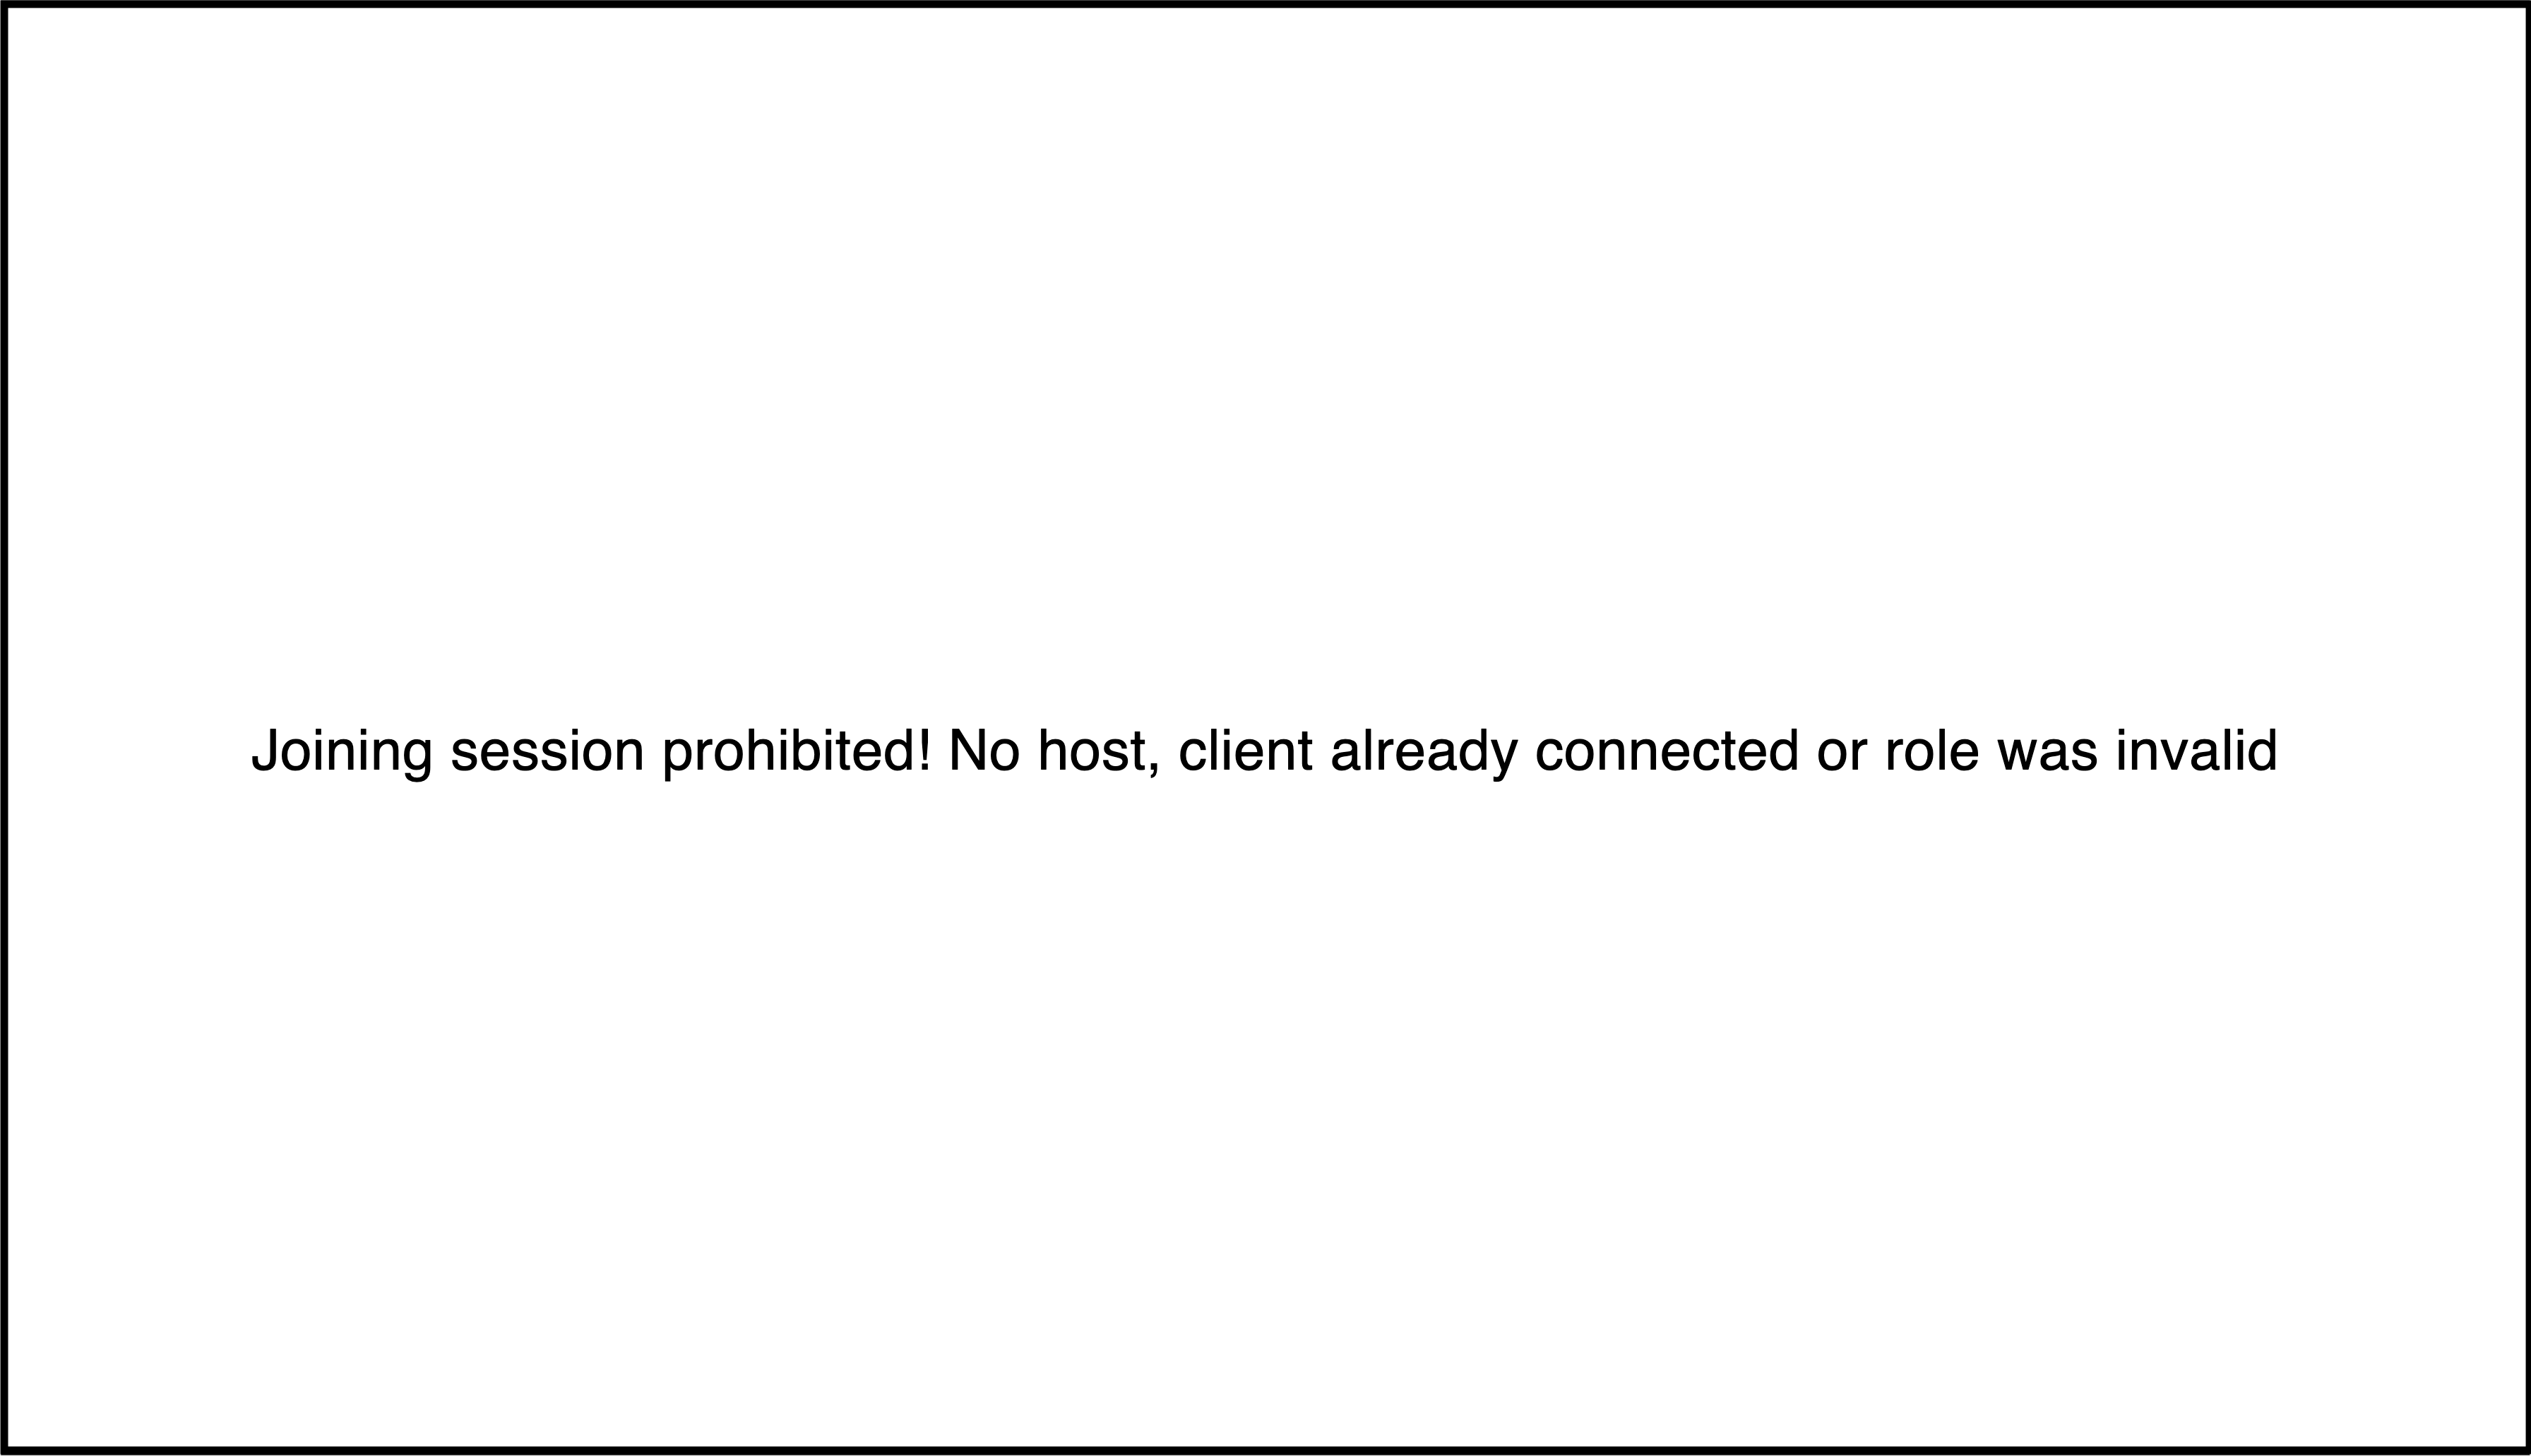
\includegraphics[width=0.6\textwidth]{images/WelcomeScreenInvalid.png}
    \caption{When trying to connect}
\end{figure}
If a user is already connected to the server, any subsequent user who scans the QR code will see 
a different screen on their device, informing them that the \textbf{session is currently occupied}.
\section{Modes}

\subsection{QR Code - Integration}
QR codes play a central role in how devices connect within \textbf{SeQG}. 
They are used as a simple and intuitive way to link a user's device to an active session. 
When a session is started, the application generates a QR code containing a unique link. 
This link includes a hidden session identifier that tells the system, which session the user can connect to.
Once scanned, the device opens the link, which automatically redirects the user to the corresponding session within the app. 
The beauty of this process is that it requires almost no effort from the user, as no code or password is required. 
Everything happens in just a few seconds by scanning the QR code.

\subsection{Communication with Backend}
The \textbf{SeQG} frontend communicates with the backend through WebSockets to enable real-time, bidirectional data exchange. 
Here we differentiate between client and host frontend.
The host frontend must stay in constant connection with the backend, while a session is active, whereas the client frontend needs to connect only once. 
Before the client can connect, the host frontend must first request a JWT token and then connect to the backend with this token.
As the user joins a session, the client's frontend uses the previously fetched JWT token from the host's frontend and connects to the backend, via the URL saved in the QR Code. 
While connecting, the client's frontend emits an ''register'' event containing:
\begin{itemize}
    \item the token from the URL
    \item a role
    \item the user's unique ID from localStorage (if private-mode)
\end{itemize}
If the session is valid and the user is allowed to join, they're granted access and the interaction begins. 
If not, they receive a ''already\_connected'' message, which can then be handled as an invalid user.
This approach makes it easy to manage users in real time.
\subsection{Guest Mode}
Guest Mode is designed for quick, one-time participation without any setup or login. 
It allows users to access a session instantly without any user data being stored. 
When someone joins a session in Guest Mode, the application automatically generates a temporary user identity and stores it locally in the browser. 
This identity helps the system recognize the user during the session. 
Guest users have full access to participate in the session’s activities, but their presence is temporary and not tied to any personal information. 
Once the session ends or the browser is closed, the user effectively disappears from the system’s memory.
This mode is ideal for situations where users are not expected to return.

\subsection{Private Mode}
Private Mode offers a more structured and secure way to connect to a session. 
It is used when a user scans a QR code that links to a specific, private session. 
This link contains a hidden token that identifies the session and grants access to it. 
When the user opens the link, the application uses this token to establish a secure connection with the backend system. 
At the same time, the user's device is assigned a unique identifier, which is stored locally and remains available for future sessions on the same device. 
This allows the system to recognize returning users, maintain a consistent identity across multiple sessions, and apply session-specific rules or roles. 
The connection is verified before granting access — so users without the correct token or link will be blocked.
\subsection{Question Types}
SeQG has \textbf{six question types implemented}, enhancing the user's gamified experience with a dynamic, entertaining
app. Each of these question types has been implemented with visual animations depending on the correctness of
the answer and each one of them has an explanation generated by the LLM in case the user answered incorrectly.
The six question types are:
\begin{itemize}[nosep]
    \item \textbf{Single choice} 
    \item \textbf{Multiple choice} 
    \item \textbf{Think event} 
    \item \textbf{Drag \& drop}
    \item \textbf{Sorting}
    \item \textbf{Line-connect}
\end{itemize}

\pagebreak
\subsubsection{Single choice}
In this question type, the user is offered \textbf{two possible solutions} and has to select the correct answer. Once they
touch on the desired answer, the correct answer will be highighted in green. If they have failed, an instant LLM explanation
will be fetched on the same screen for the user to learn:
\begin{figure}[htbp]
    \centering
    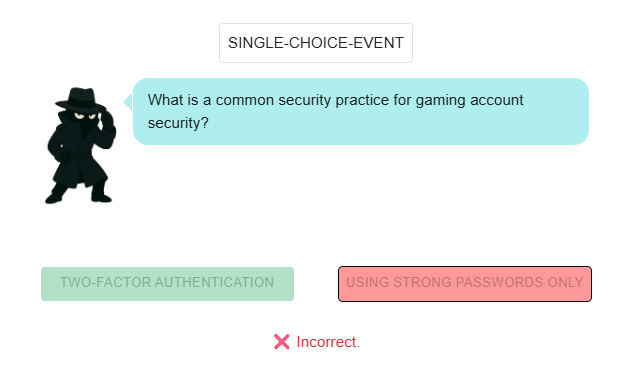
\includegraphics[width=0.5\textwidth]{images/Single_Choice.png}
\end{figure}

\subsubsection{Multiple choice}
Here the user is given \textbf{between two and four possible solutions} and has to select \textbf{all} correct answers. Once every
correct asnwer is selected, the must press the submit button:
\begin{figure}[htbp]
    \centering
    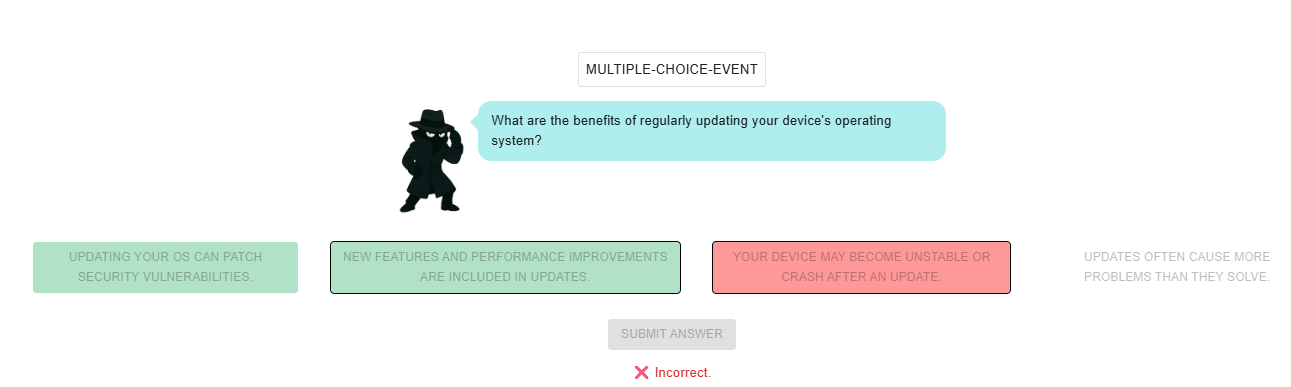
\includegraphics[width=1\textwidth]{images/Multiple_Choice.png}
\end{figure}

\subsubsection{Think Event}
In the think event, the user must think about the possible answer to the question formulated for \textbf{fifteen seconds}. Once the
time is up, they must (honestly) select whether they knew the correct answer or not:
\begin{figure}[htbp]
    \centering
    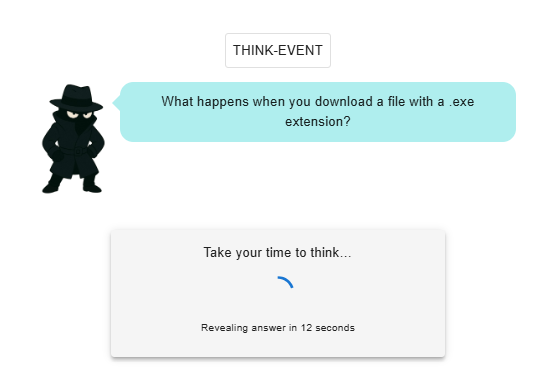
\includegraphics[width=0.45\textwidth]{images/Think_Event.png}
    \hfill
    \raisebox{-5mm}{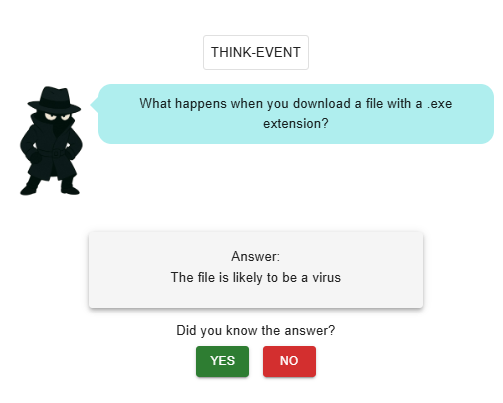
\includegraphics[width=0.45\textwidth]{images/Think_Event_2.png}}
\end{figure}
\pagebreak

\subsubsection{Drag \& Drop}
The user must drag the boxes into the \textbf{correct category}. There is also the possibility to revert the answer:
\begin{figure}[htbp]
    \centering
    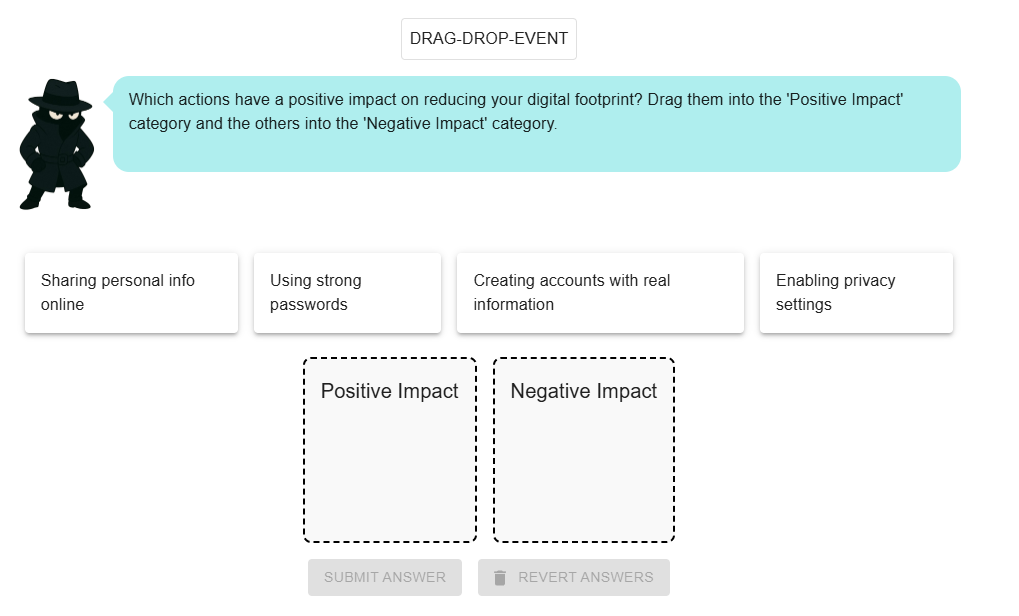
\includegraphics[width=0.8\textwidth]{images/Drag_and_Drop.png}
\end{figure}

\subsubsection{Sorting}
All the answers must be \textbf{correctly sorted}. As before, the user can return to the original order whenever they want:
\begin{figure}[htbp]
    \centering
    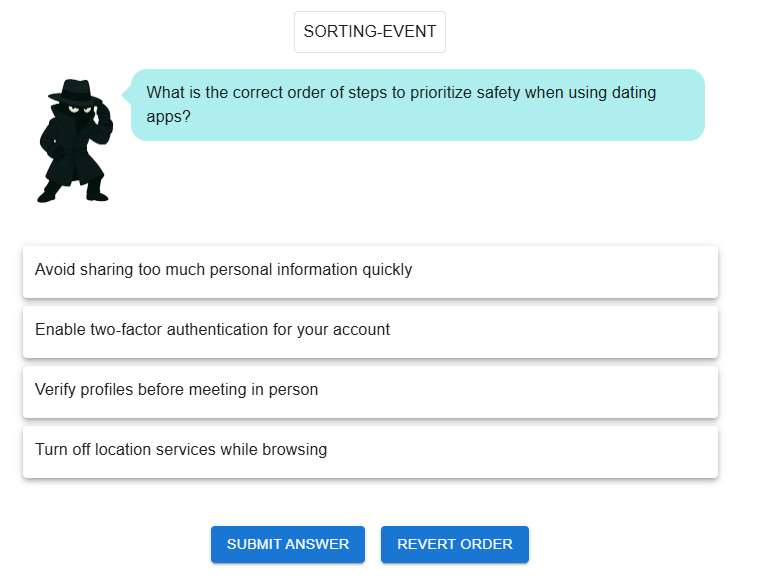
\includegraphics[width=0.6\textwidth]{images/Sorting.png}
\end{figure}
\pagebreak

\subsubsection{Line-connect}
In tis question type \textbf{an even number} of boxes is displayed, having to match each item on one side to their correspondant
on the other side. There is also the answer reversal button to start again:
\begin{figure}[htbp]
    \centering
    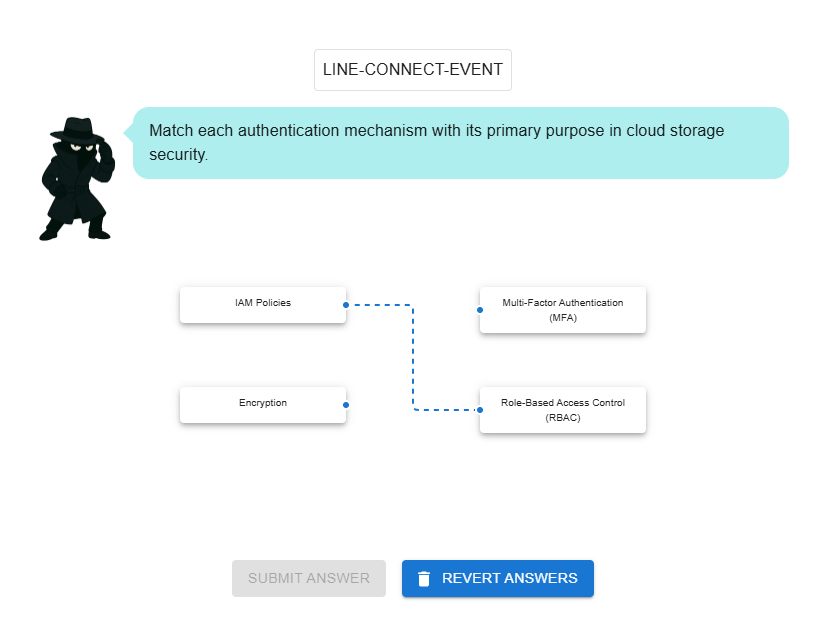
\includegraphics[width=0.8\textwidth]{images/Line_Connect.png}
\end{figure}

\subsection{Gradings}

When the user finishes their session (in both guest and private modes), a dashboard appears summarizing their \textbf{performance}. 
To enhance user feedback and engagement in SeQG, the dashboard includes radar charts assessing the user's performance 
across each specific \textbf{cybersecurity topic}, generated with Chart.js. The diagram is split into two if there are more 
than eight topics, to avoid exceeding the visual limit. The dashboard also includes \textbf{personalized feedback}, as 
shown in Figure 2.5, which highlights the user's strengths and weaker areas during their session, encouraging 
them to use SeQG again to improve their \textbf{cybersecurity awareness}. User Progress is persistently stored in a 
structured JSON format if the user started a private session, including metadata such as their userID, age, 
experience and per-topic experience.

\begin{figure}[H]
    \centering
    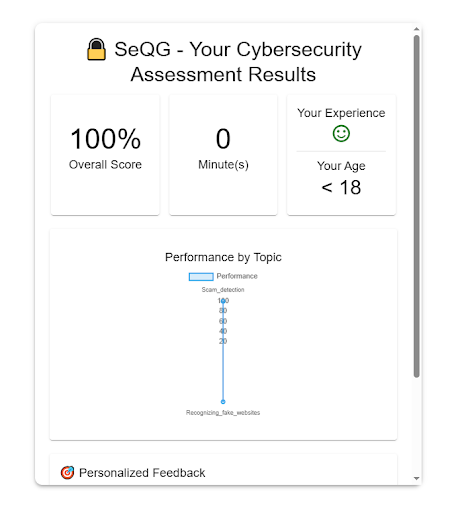
\includegraphics[width=0.4\textwidth]{images/Grading2.png}
    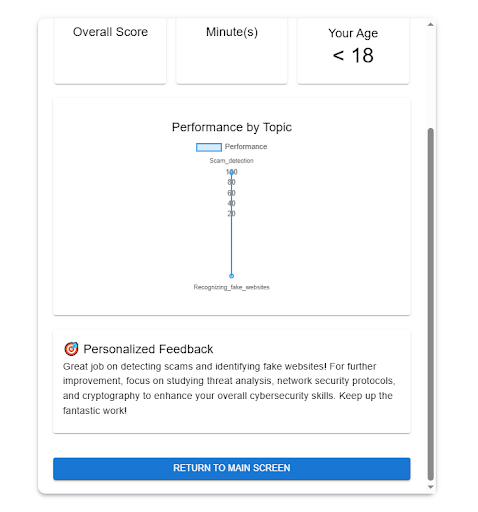
\includegraphics[width=0.4\textwidth]{images/Grading3.png}
    \caption{Dashboard}
\end{figure}

The interface also includes an inactivity timer that triggers a message in the center of the screen after 60 seconds 
of \textbf{no interaction}. The user then has 10 seconds to confirm their presence; otherwise, the session is closed and the 
system returns to the main screen.

\begin{figure}[H]
    \centering
    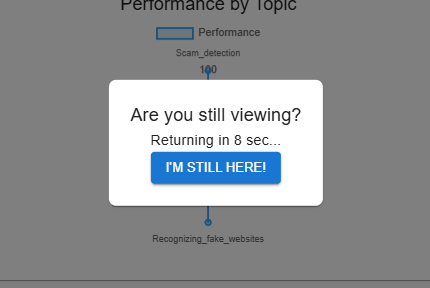
\includegraphics[width=0.35\textwidth]{images/Grading1.png}
    \caption{Inactivity timer pop-up message}
\end{figure}
\chapter{Backend}

The backend is the silent core of the entire project, which makes it possible enabling connection between the user and front end.
As the user establishes a connection to the front end, the next Backend component is made active, namely the interaction between the front end and the LLM API
After a session, our backend then also covers the safe disconnection logic and resets everything to a clean state. 

\section{QR Code - Connection}
The whole connections starts by making sure the user visits the link via. scanning the QR code.
Afterwards a link gets generated, that is unique for every session and contains a JWT token.
This token gets generated by the backend and send over to the front-end and only then the user may connect.
In that way, we make sure that no connection can be established without the user having the right to do so.
The front-end then uses this exact JWT token and only allows connections with the same token in current use.
Considering all previous steps, the actual connection logic is then handled by the users front-end, from which the device (e.g. phone) emits a ''register'' message to the backend.
This leads to the final step of the connection, where the backend receives the message and sends over the status that is appropriate for the current connection state.
If everything worked optimally the front-end gets the message ''connected'' emited from the backend. 
\subsection{Role \& Status}
First we have to define what actual roles can connect, this makes random or brute connections even harder.
Currently we have two roles, namely the ''client'' and ''host'' role.
The client is the one who connects to the host, whereas the host is the one who gives the opportunity connecting to the currently active session. \\ \\

To make sure a connection is actually valid we now discuss the part where we need to define different states helping us understanding what went pottentially wrong in a connection. \\
The following states currently in use are defined as:
\begin{itemize}
    \item \textbf{pending} - The QR Code is created and the front-end is waiting for the user to connect.
    \item \textbf{connected} - The user has successfully connected to the session and can now use the application as intended.
    \item \textbf{disconnected} - The user has disconnected from the session, either by closing the application or by a timeout.
    \item \textbf{already\_connected} - The user or a host was already connected to the backend, which moves potential intruders into a url sinkhole.
\end{itemize}
The states that should be added for a more detailed error handling are:
\begin{itemize}
    \item \textbf{no\_host} - The user tries to connect to a session that does not exist.
    \item \textbf{invalid\_role} - The user tries to connect with a role that does not exist.
\end{itemize}

\subsection{Registration}
Making the connection valid though, it is not enough to just scan the qr code.
We actually need a registration logic that makes sure that the host and client are allowed to connect.
This is done by the host front-end and clients front-end, who both need to emit a ''register'' message to the backend.
By registering, the backend recognizes if a host or client is already connected.
This makes flag handling easier, as the backend can then emit a message to the host or client front-end appropriate to the actual status.
If the user is in private mode, then we emit a special message called ''register-private'', 
which then creates a file with a unique uuid and a token in the local storage of the users browser.
This file and local storage token is only created though if the user submits his age and experience first.
Such a file would then look like this:
\begin{lstlisting}[language=json,firstnumber=1]
{
    "user_id": "abc123",
    "age": "< 18",
    "experience": 2,
    "progress": {}
}
\end{lstlisting}
Where the \textbf{user\_id} (String) is the unique identifier for the user, 
\textbf{age} (String) is the apporximate age of the user, 
\textbf{experience} (Integer) is the experience level of the user and 
\textbf{progress} (Object) is an object that will hold the progress of the user with counted questionTypes and if they where answered correctly.

\section{API Calls}
In actuality currently there exist four API calls the qr-code backend is handling.
\begin{itemize}
    \item \textbf{/connect/host} - This is the call that is used by the host to connect to the backend and receiving the JWT token.
    \item \textbf{/disconnect/all} - This call is used by the client or host to close the current session.
    \item \textbf{/private/user-data/:userId} - Here we get the private-user data from the backend, which is already stored (currently only age and experience).
    \item \textbf{/private/saveAgeAndExprience} - This call is used to save the age and experience of the user in a private session.
\end{itemize}
Adding more API calls is possible, but currently not needed.
If one shall adjust those calls then only in the matter of better verification, so that no workaround allows to use these API calls without the right to do so.
\section{LLM - Connection}
Before the user gets to actually answer questions provided by the LLM, he needs to submit his age and experience, if not already done.
Only then the questions will start to get fetched from the LLM API.
But this is not happening directly, for which we also implemented a little backend, that needs to be started, which then handles all needed API calls.
Currently though the backend is not protected against calls from outside, so it is not recommended to run it on a public server.
One might first want to implement some kind of authentication, before doing so. 
The same goes for the LLM API, as it is a Ollama Backend that runns openly.
Here we also recommend to implement authentication procedures, such as private keys or doing network segmentation only for the API, to prevent unwanted access.

\subsection{Tips}
To catch a potential users attention, we decided to use Tips and eye catching messages on our main screen.
This shall then make the users interest rise about our PSUI and let him or her approach our Public Display.
These tips are getting fetched from the LLM API.
In case of server connection issue, we have a fallback mechanism that uses locally saved tips.
Later on in the future, one may also add not only tips, but also current news in cybersecurity and generally speaking of security awareness.
There are multiple API available, even for free, that allow to fetch current events in cybersecurity.

\subsection{Questions}
Here we differentiate between the two modes, as one of them has a userId and the other one does not.
Considering that, lets first look at the guest-mode question API request.
For that we have prepared a prompt and a list of topics from which the llm can choose.
Both of them are stored in the backend folder.
From here on we directly pass arguments into the prompt such as: age, experience and the topic.
When we are done, we simply send over the whole prompt to the LLM API, which then responds with a specific \textbf{json} format.
The \textbf{json} format is then parsed and send over to the host front end.
The formatted \textbf{json} respond then, represents this structure:
\begin{lstlisting}[language=json,firstnumber=1]
{
    "question": ... ,
    "option_s": ... ,
    "dropZones": ... ,
    "correctAnswer_s": ... ,
    "topic": ... ,
    "questionType": ...
}
\end{lstlisting}
Each one having there own meaning.
\begin{itemize}
    \item \textbf{question}: The question that the user has to answer (String).
    \item \textbf{option\_s}: The options that the user can choose from (String array).
    \item \textbf{dropZones}: Represent drop zones in a drag \& drop event, where the user can drag and drop the options (String array).
    \item \textbf{correctAnswer\_s}: Correct answers for the question (String array).
    \item \textbf{topic}: The overall topic of the question (String).
    \item \textbf{questionType}: The event-type of the question (String).
\end{itemize}

\subsection{Explanation}
In the explanation we actually dont need to differentiate between the two modes, as the explanation should be universal.
There may be a critical moment where one might think to add some extra explanation features for the private mode, but we did not implement that.
As we have fetched a question from the LLM API we can refeed it with almost the same provided json format.
In our case we only need the question and the correctAnswer\_s aswell as a boolean telling the LLM we did indeed answer the question incorrectly. \\
When we do answer correctly there is no need to explain the question, as the user already knew the answer (hopefully did not guess).
This means we have a simple return format for our explanation, because in the end we only need the explanation text. \\
Therefore our \textbf{json} format looks like this:
\begin{lstlisting}[language=json,firstnumber=1]
{
    "explanation": ... 
}
\end{lstlisting}
Where the \textbf{explanation} (String) is the text that the LLM provides us with.

\pagebreak
\subsection{Saving Answers}
When the user enters the guest mode, we do not save anything but rather do a local session with grading at the end.
However, when the user enters the private mode, we do save the answers, so that his or her previously answered questions can be taken into account.
This makes the LLM way more personalized and the user can also see his or her progress eventually.
The main idea is, that we get the Questiontype from the LLM API.
After that we add to our autogenerated file with the userId as its filename, the current Questiontype.
For the final part, we increase a counter for the correctly answered questions according to the Questiontype.
If the user indeed answered the question correctly, we increment by one, otherwise not.
The total amount of questions is also saved for each Questiontype.
This amount always gets incremented by one, no matter the correctness of the answer. \\
In general a progress output may look like this:
\begin{lstlisting}[language=json,firstnumber=1]
{
    ... ,
    "progress": {
        "passwords": {
            "correct": 0,
            "total": 1
        },
        "camera_microphone_access": {
            "correct": 0,
            "total": 1
        },
        "kids_online_safety": {
            "correct": 2,
            "total": 2
        }
  }
}
\end{lstlisting}
Which would mean that in total the user has answered 4 questions, of which he answered 2 correctly.

\subsection{Feedback}
The moment the user decides that he or she has had enough of the questions, one can request a feedback.
This feedback is then generated by the LLM API and sent over to the front end.
The user has now the oppertunity to read the feedback and then decide for himself learning more about a topic or not.
Feedbackwise we offer a spider chart limited to the maximum amount of 8 topics, where we define from 0 to a 100 percent how well the user did in each topic.
Aswell as a specificly generated text, that gives the user a more detailed overview of his or her performance.
Afterwards the user can disconnect from the session or do nothing as the session will automatically disconnect after a certain amount of time.

\section{Anti-Breaching Sessions}
As every server, that is reachable from the internet or inside a local network, we need to make sure, that we are as secure as possible.
For that we implemented a simple anti-breaching session logic.
Everytime a user connects to the backend we check if someone is already connected (max amount of client: 1, host: 1).
Therefore moving the unwanted user into a url sinkhole.
This means that refreshing the page will keep you on a prohibited url where one cannot do anything, which eases the backend servers capacity.
Additionally to that we have a structure, where even if an attacker gets the information about the current session, he cannot make anything of it.
The actual data that is stored from the user does not contain any sensitive information, 
but rather a unique userId, a rough approximate of the age aswell as the experience level, the user provided us with.
Additionally the JWT token is only valid for a certain amount of time, which makes it even harder to breach the session.
Though our application is not perfect and we do not claim it to be, we still try to make it as secure as possible.
One can for example try to impersonate a user by storing the userId in his or her own local storage, this would mean, that the attacker may use the interface as
the pronounced user.
However the attacker also has to be motivated to then answer questions for the user, which he or her is impersonating.
This has no actual benefit for the attacker.
We also do something that is almost bullet proof, so that even if an attacker mages to connect to the session there is nothing the attacker can do.
As the QR Code is generated the user scans it.
In that Moment the file is being created or reused from the connected user.
Even if the attacker tries to connect now he or her will be send to the sinkhole as we remember the first user that connected with his or her specific userId.
Therefore making sure the file of the user is safe and not touchable by a potential attacker.

\section{File Cleansing}
As the user logs into the private mode, we create a file, but how do we remove it again?
There are alot of ways one could do so, but most of them require some interaction.
Therfore we decided that a simple python script, running maybe once a month, shall remove all files that are older than 30 days.
This may seem unfortunate for the user as his progress is lost after one month but for the servers memory sake we need a way to remove files after a certain amount of time.
If we try to keep them forever this may lead to dead files, as users may never return or users often delete there browser cache, maybe even change there browser.
All that has influence on how the files are getting accessed and therefore we really need a way to remove them.
The script itself is in the backend folder called ''checkFiles.py''.


\end{document}